\documentclass[a4paper,12pt]{report}
\usepackage{mathtext}
\usepackage[T2A]{fontenc}
\usepackage[utf8]{inputenc}
\usepackage[english,russian]{babel}
\usepackage{geometry}
\usepackage{listings}
\usepackage{amsmath}
\geometry{top=2cm}
\usepackage{titlesec}
\usepackage{color}
\usepackage{pgfplots}
\usepackage{filecontents}
\usetikzlibrary{datavisualization}
\usetikzlibrary{datavisualization.formats.functions}
\usepackage{caption}
\DeclareCaptionFont{white}{\color{white}}
\DeclareCaptionFormat{listing}{\colorbox{gray}{\parbox{\textwidth}{#1#2#3}}}
\captionsetup[lstlisting]{format=listing,labelfont=white,textfont=white}

% Для листинга кода:
\lstset{ %
language=Python,                 % выбор языка для подсветки
basicstyle=\small\sffamily, % размер и начертание шрифта для подсветки кода
numbers=left,               % где поставить нумерацию строк (слева\справа)
numberstyle=\tiny,           % размер шрифта для номеров строк
stepnumber=1,                   % размер шага между двумя номерами строк
numbersep=-5pt,                % как далеко отстоят номера строк от подсвечиваемого кода
showspaces=false,
backgroundcolor=\color{white},         
showstringspaces=false,      % показывать или нет пробелы в строках
showtabs=false,             % показывать или нет табуляцию в строках
frame=single,              % рисовать рамку вокруг кода
tabsize=2,                 % размер табуляции по умолчанию равен 2 пробелам
captionpos=t,              % позиция заголовка вверху [t] или внизу [b] 
breaklines=true,           % автоматически переносить строки (да\нет)
breakatwhitespace=false, % переносить строки только если есть пробел
escapeinside={\%*}{*)},   % если нужно добавить комментарии в коде
	    keywordstyle=\color{blue}\ttfamily,
	    stringstyle=\color{red}\ttfamily,
	    commentstyle=\color{green}\ttfamily,
	    morecomment=[l][\color{magenta}]{\#},
	    columns=fullflexible   % если нужно добавить комментарии в коде
}

% Для измененных титулов глав:
\definecolor{gray75}{gray}{0.75} % определяем цвет
\newcommand{\hsp}{\hspace{20pt}} % длина линии в 20pt
% titleformat определяет стиль
\titleformat{\chapter}[hang]{\Huge\bfseries}{\thechapter\hsp\textcolor{gray75}{|}\hsp}{0pt}{\Huge\bfseries}


% Графики
\begin{filecontents}{StandardEven.dat}
100 0.1575000
200 1.2500000
300 4.3307813
400 10.3662500
500 20.4650000
600 35.1328125
700 55.8004688
800 86.1578125
900 121.7937500
1000 167.6281250
\end{filecontents}

\begin{filecontents}{VinogradEven.dat}
100 0.1857813
200 1.4631250
300 5.0285937
400 12.1034375
500 23.8662500
600 42.7621875
700 68.0123437
800 104.2671875
900 148.9187500
1000 204.6281250
\end{filecontents}

\begin{filecontents}{OptimizedEven.dat}
100 0.0982813
200 0.7660938
300 2.7096875
400 6.7565625
500 13.5250000
600 23.9798438
700 38.5164063
800 59.3812500
900 85.0656250
1000 118.0187500
\end{filecontents}

\begin{filecontents}{StandardOdd.dat}
101 0.1671875
201 1.2984375
301 4.4859375
401 10.8093750
501 20.8265625
601 36.9187500
701 57.3937500
801 85.7406250
901 122.8031250
1001 167.6046875
\end{filecontents}

\begin{filecontents}{VinogradOdd.dat}
101 0.2000000
201 1.5187500
301 5.1656250
401 12.4781250
501 24.4750000
601 44.0031250
701 70.3046875
801 104.2187500
901 149.4390625
1001 205.3968750
\end{filecontents}

\begin{filecontents}{OptimizedOdd.dat}
101 0.1000000
201 0.7875000
301 2.7765625
401 6.9390625
501 13.9140625
601 24.9343750
701 39.9531250
801 60.1828125
901 86.1062500
1001 119.3390625
\end{filecontents}


\begin{document}
\begin{titlepage}
	\centering
	{\scshape\LARGE МГТУ им. Баумана \par}
	\vspace{4cm}
	{\scshape\Large Лабораторная работа №2\par}
	\vspace{0.5cm}	
	{\scshape\Large По курсу: "Анализ алгоритмов"\par}
	\vspace{2cm}
	{\huge\bfseries Алгоритмы умножения матриц\par}
	\vspace{3cm}
	\Large Работу выполнил: Луговой Дмитрий, ИУ7-51Б\par
	\vspace{0.5cm}
	\Large Преподаватель:  Волкова Л.Л.\par

	\vfill
	\large \textit {Москва, 2019} \par
\end{titlepage}

\setcounter{page}{2}

\tableofcontents

\newpage
\chapter*{Введение}
\addcontentsline{toc}{chapter}{Введение}
\hspace{0.6cm} \textbf{Целью} данной лабораторной работы является исследование существующих алгоритмов умножения матриц и их трудоемкости.\\
Примем следующую модель вычислений:
\begin{enumerate}
\item Трудоемкость базовых операций\\
Операции $+$, $-$, $*$, $/$, $\%$, $=$, $>$, $<$, $\leq$, $\geq$, $==$, $\neq$, $[\space]$, $+=$, $-=$ - имеют стоимость 1.
\item Трудоемкость условного перехода\\
Условный переход имеет стоимость 0, при этом оцениваем расчет условия:
\begin{align*}
& if \ (n \ \% \ 2 \ == \ 1)\\
& \{\\
&  \ \ \ \ // \ Тело \ 1\\
& \}\\
& else \\
& \{\\
& \ \ \ \ // \ Тело \ 2 \\
& \}
\end{align*}
\[ f_{if} = f_{условия} + \begin{cases} f_{тело \ 1},& при\ нечетном\ N\\ f_{тело \ 2},& при\ четном\ N \end{cases}\\ \]


\item Трудоемкость цикла $for$\\

$f_{цикла} = f_{инициализации} + f_{сравнения} + N(f_{тела} + f_{инкремента} + f_{сравнения})$,

где $N$ - число повторений цикла.
\end{enumerate}
\newpage
\textbf{\LARGE Задачи работы}\\\\
Задачами данной лабораторной являются:
\begin{enumerate}
  	\item Реализовать следующие алгоритмы умножения матриц:
  	\begin{itemize}
		\item Стандартный алгоритм
		\item Алгоритм Винограда
		\item Оптимизированный алгоритм Винограда
	\end{itemize}
	\item Проанализировать трудоемкость данных алгоритмов
	\item Провести эксперименты с замерами времени  
\end{enumerate}


\chapter{Аналитическая часть}
\hspace{0.6cm}В этом разделе содержатся описания умножения матриц.

\section{Стандартный алгоритм}
\hspace{0.6cm}Пусть даны две прямоугольные матрицы A и B размерностей $m \times n$ , $n \times q$ соответственно:

\[
A = 
  \begin{bmatrix} 
    a_{11} & a_{12} & \cdots & a_{1n} \\
    a_{21} & a_{22} & \cdots & a_{2n} \\ 
    \vdots & \vdots & \ddots & \vdots \\ 
    a_{m1} & a_{m2} & \cdots & a_{mn}
  \end{bmatrix},\;\;\;
\]
\[
B =   
  \begin{bmatrix} 
    b_{11} & b_{12} & \cdots & b_{1q} \\
    b_{21} & b_{22} & \cdots & b_{2q} \\ 
    \vdots & \vdots & \ddots & \vdots \\ 
    b_{n1} & b_{n2} & \cdots & b_{nq}.
  \end{bmatrix}.
\]
Тогда матрица C размерностью $m \times q$
\[
C = 
  \begin{bmatrix} 
    c_{11} & c_{12} & \cdots & c_{1q} \\
    c_{21} & c_{22} & \cdots & c_{2q} \\ 
    \vdots & \vdots & \ddots & \vdots \\ 
    c_{m1} & c_{m2} & \cdots & c_{mq}
  \end{bmatrix},
\]
в которой:\\

$c_{ij} = \sum_{k=1}^n a_{ik}b_{kj} \;\;\; \left(i=1, 2, \ldots m;\; j=1, 2, \ldots q \right)$\\

называется их произведением. Операция умножения двух матриц выполнима только в том случае, если число столбцов в первом сомножителе равно числу строк во втором; в этом случае говорят, что матрицы согласованы. В частности, умножение всегда выполнимо, если оба сомножителя — [[Квадратная матрица|квадратная матрица]] одного и того же порядка. 

Таким образом, из существования произведения AB вовсе не следует существование произведения BA

\section{Алгоритм Копперсмита-Винограда}
\hspace{0.6cm} \textbf {Алгоритм Копперсмита—Винограда} — алгоритм умножения матриц, предложенный в 1987 году Д. Копперсмитом и Ш. Виноградом. В исходной версии асимптотическая сложность алгоритма составляла $O(n^{2,3755})$, где n — размер стороны матрицы. Алгоритм Копперсмита—Винограда, с учетом серии улучшений и доработок в последующие годы, обладает лучшей асимптотикой среди известных алгоритмов умножения матриц.\\
Если посмотреть на результат умножения двух матриц, то видно, что каждый элемент в нем представляет собой скалярное произведение соответствующих строки и столбца исходных матриц. Можно заметить также, что такое умножение допускает предварительную обработку, позволяющую часть работы выполнить заранее. 
Рассмотрим два вектора
$V = (v1, v2, v3, v4)$ и
$W = (w1, w2, w3, w4)$.
Их скалярное произведение равно: 
$V * W = v1w1 + v2w2 + v3w3 + v4w4$.
Это равенство можно переписать в виде: 
$V * W = (v1 + w2)(v2 + w1) + (v3 + w4)(v4 + w3) - v1v2 - v3v4 - w1w2 - w3w4$.

Кажется, что второе выражение задает больше работы, чем первое: вместо четырех умножений мы насчитываем их шесть, а вместо трех сложений - десять. Однако выражение в правой части последнего равенства допускает предварительную обработку: его части можно вычислить заранее и запомнить для каждой строки первой матрицы и для каждого столбца второй. На практике это означает, что над предварительно обработанными элементами нам придется выполнять лишь первые два умножения и последующие пять сложений, а также дополнительно два сложения.

\chapter{Конструкторская часть}
\hspace{0.6cm}В этом разделе содержатся cхемы алгоритмов умножения матриц и подсчет трудоемкости.
\newpage
\section{Схемы алгоритмов}

\hspace{0.6cm}На Рис.2.1 и 2.2 представлена схема стандартного алгоритма умножения матриц.
\begin{figure}[ht!]
\center{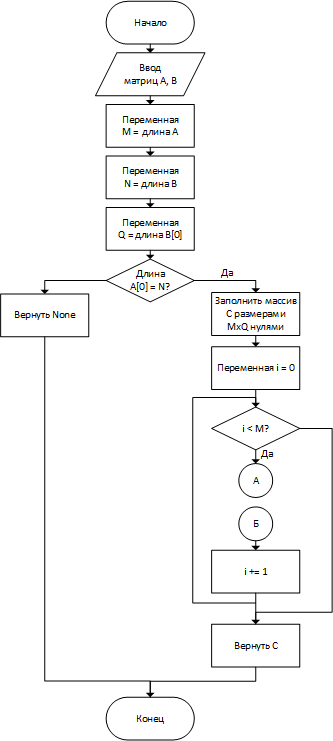
\includegraphics[scale=1]{Standart1.png}}
\caption{Стандартный алгоритм умножения матриц}
\newpage
\end{figure}
\newpage
\begin{figure}[ht!]
\center{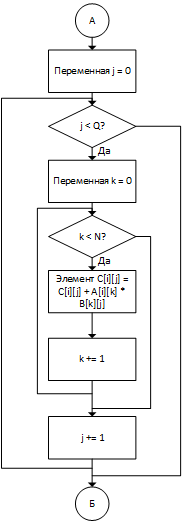
\includegraphics[scale=1]{Standart2.png}}
\caption{Стандартный алгоритм умножения матриц(продолжение)}
\end{figure}
\newpage
На Рис.2.3, 2.4, 2.5 и 2.6 представлена схема алгоритма Винограда умножения матриц.
\begin{figure}[ht!]
\center{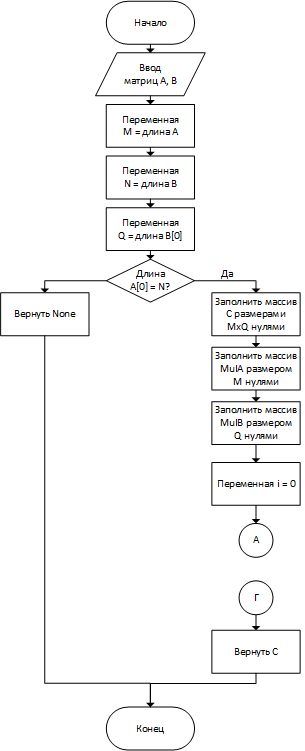
\includegraphics[scale=1]{Vinograd1.png}}
\caption{Алгоритм Винограда умножения матриц}
\end{figure}
\newpage
\begin{figure}[ht!]
\center{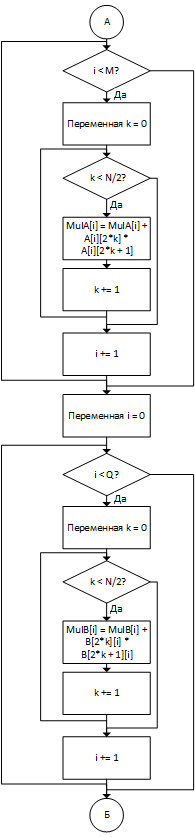
\includegraphics[scale=1]{Vinograd2.png}}
\caption{Алгоритм Винограда умножения матриц(продолжение 1)}
\end{figure}
\newpage
\begin{figure}[ht!]
\center{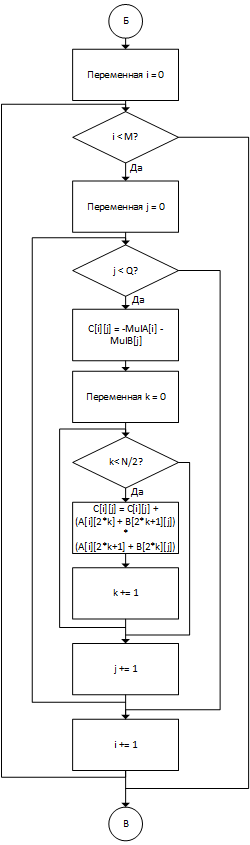
\includegraphics[scale=1]{Vinograd3.png}}
\caption{Алгоритм Винограда умножения матриц(продолжение 2)}
\end{figure}
\newpage
\begin{figure}[ht!]
\center{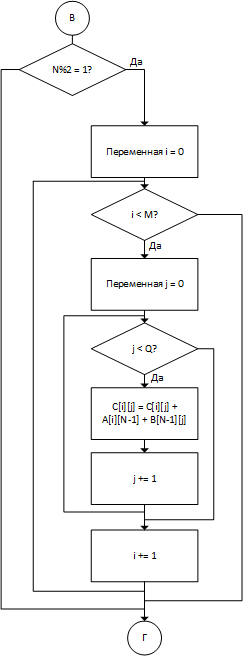
\includegraphics[scale=1]{Vinograd4.png}}
\caption{Алгоритм Винограда умножения матриц(продолжение 3)}
\end{figure}
\newpage

На Рис.2.7, 2.8, 2.9 и 2.10 представлена схема оптимизированного алгоритма Винограда умножения матриц.

\begin{figure}[ht!]
\center{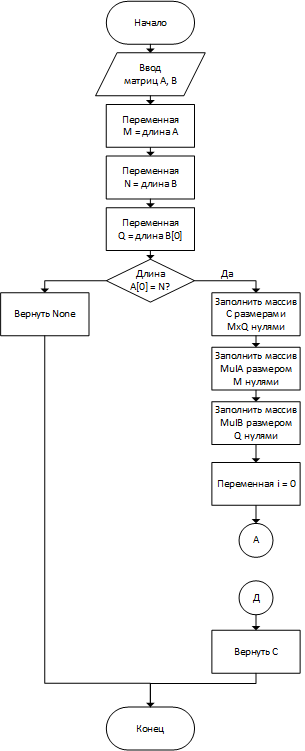
\includegraphics[scale=1]{Optimized1.png}}
\caption{Оптимизированный алгоритм Винограда умножения матриц}
\end{figure}

\newpage

\begin{figure}[ht!]
\center{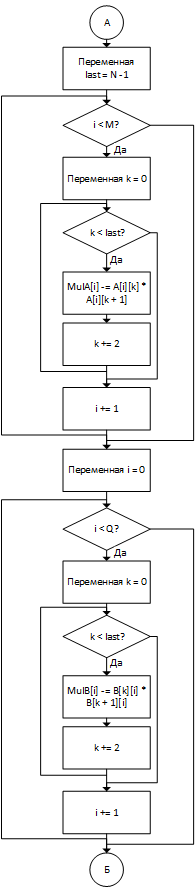
\includegraphics[scale=0.9]{Optimized2.png}}
\caption{Оптимизированный алгоритм Винограда умножения матриц(продолжение 1)}
\end{figure}

\newpage

\begin{figure}[ht!]
\center{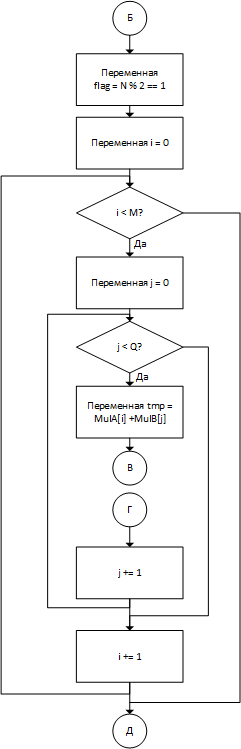
\includegraphics[scale=1]{Optimized3.png}}
\caption{Оптимизированный алгоритм Винограда умножения матриц(продолжение 2)}
\end{figure}

\newpage

\begin{figure}[ht!]
\center{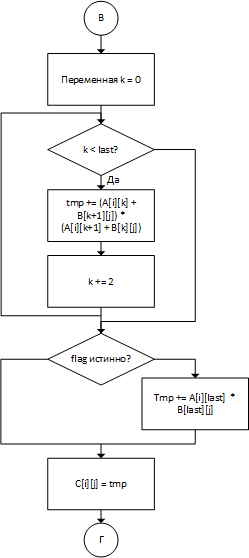
\includegraphics[scale=1]{Optimized4.png}}
\caption{Оптимизированный алгоритм Винограда умножения матриц(продолжение 3)}
\end{figure}

\newpage

\section{Расчет трудоемкости}

\hspace{0.6cm}Пусть заданы матрицы размерами $m \times n$ , $n \times q$. Используя модель вычислений, заданную ранее, произведем подсчет трудоемкости алгоритмов умножения матриц:
\begin{itemize}

\item Стандартный алгоритм
\[
f_{стд} = 2 + M(2 + 2 + Q(2 + 2 + N(2 + 8 + 1 + 1 + 1))) = 13MNQ + 4MQ + 4M + 2 \approx 13MNQ 
\]

\item Алгоритм Винограда
\begin{align*}
& f_{I} = 2 + M(2 + 3 + \frac{N}{2} (3 + 1 + 6 + 2 + 3)) = \frac{15}{2} MN + 5M + 2\\
& f_{II} = 2 + Q(2 + 3 + \frac{N}{2} (3 + 1 + 6 + 2 + 3)) = \frac{15}{2} QN + 5Q + 2\\
& f_{III} = 2 + M(2 + 2 + Q(2 + 7 + 3 + \frac{N}{2}(3 + 6 + 17))) = 13MNQ + 12 MQ + 4M + 2\\
& f_{IV} = 2 + \left[
	\begin{array}{ccc}
     0, & N \ четное \\
     12MQ + 4M + 2,  & N \ нечетное \\
  \end{array}
  \right.\\
\end{align*}
\begin{multline*} 
f_{вин} = f_{I} + f_{II} + f_{III} + f_{IV} = \frac{15}{2} MN + \frac{15}{2} QN + 9M + 8 + 5Q \\ + 13MNQ + 12MQ + \left[
	\begin{array}{ccc}
     0, & N \ четное \\
     12MQ + 4M + 2,  & N \ нечетное \\
  \end{array}
  \right. \approx 13MNQ
\end{multline*}

\item Оптимизированный алгоритм Винограда
\begin{align*}
& f_{I}^{*} = 2 + M(2 + 2 + \frac{N}{2} (2 + 1 + 5 + 1 + 1)) =  5MN + 4M + 2\\
& f_{II}^{*} =  2 + Q(2 + 2 + \frac{N}{2} (2 + 1 + 5 + 1 + 1)) =  5QN + 4Q + 2\\
& f_{III}^{*} = 5 + 2 + M(2 + 2 + Q(2 + 4 + 2 + \frac{N}{2}(2 + 14) + 1 + 3 + \left[
	\begin{array}{ccc}
     0, & N \ четное \\
     6,  & N \ нечетное \\
  \end{array}
  \right.)) = \\ 
  & = 7 + 4M + 12MQ + 8MNQ + \left[
	\begin{array}{ccc}
     0, & N \ четное \\
     6MQ,  & N \ нечетное \\
  \end{array}
  \right.
\end{align*}
\begin{multline*} 
f_{вин}^{*} = f_{I}^{*} + f_{II}^{*} + f_{III}^{*} = 5MN + 8M + 11 + \\5QN + 4Q + 12MQ + 8MNQ + \left[
	\begin{array}{ccc}
     0, & N \ четное \\
     6MQ,  & N \ нечетное \\
  \end{array}
  \right. \approx 8MNQ
\end{multline*}
\end{itemize}

Как видно из вычислений, наиболее эффективным по трудоемкости является оптимизированный алгоритм Винограда. 
\newpage
Трудоемкость удалось снизить за счет следующих оптимизаций:
\begin{enumerate}
\item Замена $C[i][j] = C[i][j] + \ldots$ на $C[i][j] \text{+=} \ldots$
\item Замена цикла по $k$ от $0$ до $N/2$ с шагом $1$ на цикл от $0$ до $N$ с шагом $2$, что убрало лишние умножения на 2
\item Элементы $MulA$ и $MulB$ сразу высчитываются отрицательными, что убирает 1 операцию отрицания в цикле
\item Замена $C[i][j] = \ldots$ в цикле по $k$ на буферную переменную, что убирает 2 операции индлексирования во внутреннем цикле, но добавляет С[i][j] = tmp во внешний цикл
\item Перенос проверки четности внутрь основного цикла, что ухудшило лучший случай, но улучшило худший
\item Вычисление условия четности и значения $N-1$, тем самым улучшая и лучший, и худший случаи
\end{enumerate}
\chapter{Технологическая часть}
\hspace{0.6cm}В данном разделе приведены требования к программнму обеспечению, средства реализации и листинги кода
\section{Требования к ПО}

\hspace{0.6cm}На вход поступают две целочисленные матрицы, на выходе должен возвращаться результат их умножения, либо сообщение о невозможности их умножения.
	

\section{Средства реализации}
\hspace{0.6cm}Для реализации представленных алгоритмов был выбран язык Python. Время работы алгоритмов было замерено с помощью функции process\_time() из библиотеки time.

\section{Листинги кода}

\hspace{0.6cm}В Листинге 3.1 показана реализация стандартного алгоритма умножения матриц.

\begin{lstlisting}[caption=Функция стандартного умножения матриц]
  def standard_multiply(a, b):
      m = len(a)
      n = len(b)
      if m == 0 or n == 0 or len(a[0]) != n:
          return None
      q = len(b[0])
      c = [[0 for i in range(q)] for j in range(m)]
      for i in range(m):
          for j in range(q):
              for k in range(n):
                  c[i][j] = c[i][j] + a[i][k] * b[k][j]
      return c
\end{lstlisting}
\newpage
В Листинге 3.2 показана реализация алгоритма Винограда умножения матриц.
\begin{lstlisting}[caption=Функция умножения матриц алгоритмом Винограда]
  def vinograd_multiply(a, b):
      m = len(a)
      n = len(b)
      if m == 0 or n == 0 or len(a[0]) != n:
          return None
      q = len(b[0])
      # Part I
      r = n // 2
      mul_a = [0] * m
      for i in range(m):
          for j in range(r):
              mul_a[i] = mul_a[i] + a[i][j * 2] * a[i][j * 2 + 1]

      # Part II
      mul_b = [0] * q
      for i in range(q):
          for j in range(r):
              mul_b[i] = mul_b[i] + b[j * 2][i] * b[j * 2 + 1][i]

      # Part III
      c = [[0 for i in range(q)] for j in range(m)]
      for i in range(m):
          for j in range(q):
              c[i][j] = -mul_a[i] - mul_b[j]
              for k in range(r):
                  c[i][j] = c[i][j] + (a[i][2 * k] + b[2 * k + 1][j]) \
                            * (a[i][2 * k + 1] + b[2 * k][j])

      # Part IV
      if n % 2 == 1:
          for i in range(m):
              for j in range(q):
                  c[i][j] = c[i][j] + a[i][n - 1] * b[n - 1][j]
      return c
\end{lstlisting}
\newpage
В Листинге 3.3 показана реализация оптимизированного алгоритма Винограда умножения матриц.
\begin{lstlisting}[caption=Функция умножения матриц оптимизированным алгоритмом Винограда]
  def optimized_vinograd_multiply(a, b):
      m = len(a)
      n = len(b)
      if m == 0 or n == 0 or len(a[0]) != n:
          return None
      q = len(b[0])
      last = n - 1  # Optimization for odd numbers
      # Part I
      mul_a = [0] * m
      for i in range(m):
          for j in range(0, last, 2):  # Optimization for n // 2
              mul_a[i] -= a[i][j] * a[i][j + 1]  # Optimization for negative and +=

      # Part II
      mul_b = [0] * q
      for i in range(q):
          for j in range(0, last, 2):  # Optimization for n // 2
              mul_b[i] -= b[j][i] * b[j + 1][i]  # Optimization for negative and +=

      flag = n % 2 == 1
      # Part III
      c = [[0 for i in range(q)] for j in range(m)]
      for i in range(m):
          for j in range(q):
              tmp = mul_a[i] + mul_b[j]  # Optimization for buffer
              for k in range(0, last, 2):  # Optimization for n // 2
                  tmp += (a[i][k] + b[k + 1][j]) \
                         * (a[i][k + 1] + b[k][j])  # Optimization for +=
              if flag:  # Optimization for odd numbers
                  tmp += a[i][last] * b[last][j]
              c[i][j] = tmp

      return c
\end{lstlisting}



\chapter{Экспериментальная часть}
В данном разделе приведены примеры работы программы, постановка эксперимента и сравнительный анализ алгоритмов на основе экспериментальных данных.
\section{Примеры работы}
\hspace{0.6cm}\textbf {Пример 1}\\
Матрица A:\\
1 2 3\\
4 5 6\\
Матрица B:\\
1\\
2\\
3\\
Результирующая матрица:\\
14\\
32\\

\textbf {Пример 2}\\
Матрица A:\\
5 2\\
1 4\\
Матрица B:\\\
0 3\\
-6 1\\
Результирующая матрица:\\
-12 17\\
-24 7\\

\newpage 
\textbf {Пример 3}\\
Матрица A:\\
2 7\\
1 3\\
Матрица B:\\
-3 7\\
1 -2\\
Результирующая матрица:\\
1 0\\
0 1\\

\section{Функциональное тестирование}
\hspace{0.6cm}Было проведено функциональное тестирование программы, результаты которого занесены в Таблицу 4.1,1 столбец которой - номер тестового случая, 2 и 3 столбцы - виды матриц, поступающих на вход, 4 столбец - ожидаемый результат, где $None$ означает, что матрицы несовместимы по размеру, 5 столбец - полученный результат. \\

\begin{table}[h!]
\begin{center}
\begin{tabular}{| c | c | c | c | c |}
\hline
№ & A & B & Ожидаемый результат & Полученный результат \\
\hline
1 & Случайная & Пустая & None & None\\
\hline
2 & Пустая & Случайная & None & None\\
\hline
3 & Пустая & Пустая & None & None\\
\hline
4 & Случайная & Нулевая & Нулевая & Нулевая\\
\hline
5 & Нулевая & Случайная & Нулевая  & Нулевая \\
\hline
6 & Единичная & Квадратная & B & B\\
\hline
7 & Квадратная & Единичная & A & A\\
\hline
8 & Размера $M \times N$ & Размера $M \times N$ & None & None\\
\hline
\end{tabular}
\caption{Тестовые случаи}
\end{center}
\end{table}

Программа успешно прошла все тестовые случаи, все полученные результаты совпали с ожидаемыми.

\section{Сравение алгоритмов по времени}
\hspace{0.6cm}Для экспериментов использовались матрицы, размер которых варьируется от $100 \times 100$ до $1000 \times 1000$ с шагом 100 для матриц четных размеров и от $101 \times 101$ до $1001 \times 1001$ с шагом 100 для матриц нечетных размеров. 
    Количество повторов каждого эксперимента = 100. Результат одного эксперимента рассчитывается как средний из результатов проведенных испытаний с одинаковыми входными данными.
    

\begin{figure}[ht!]
\begin{center}
\begin{tikzpicture}[scale = 1.1]
\begin{axis}[
    	axis lines = left,
    	xlabel = {Размерность матрицы},
    	ylabel = {Время(секунды)},
	legend pos=north west,
	ymajorgrids=true,
]
\addplot[color=green] table[x index=0, y index=1] {StandardEven.dat}; 
\addplot[color=red] table[x index=0, y index=1] {VinogradEven.dat};
\addplot[color=blue] table[x index=0, y index=1] {OptimizedEven.dat};
\addlegendentry{Стандартный}
\addlegendentry{Винограда}
\addlegendentry{Оптимизированный}
\end{axis}
\end{tikzpicture}
\caption{Алгоритмы умножения матриц(четных размеров)}
\end{center}
\end{figure}

На Рис. 4.1 видно, что оптимизированный алгоритм Винограда превосходит стандартный алгоритм умножения на $\approx 30\%$, а алгоритм Винограда на $\approx45\%$.

\begin{figure}[ht!]
\begin{center}
\begin{tikzpicture}[scale = 1.1]
\begin{axis}[
    	axis lines = left,
    	xlabel = {Размерность матрицы},
    	ylabel = {Время(секунды)},
	legend pos=north west,
	ymajorgrids=true,
]
\addplot[color=green] table[x index=0, y index=1] {StandardOdd.dat}; 
\addplot[color=red] table[x index=0, y index=1] {VinogradOdd.dat};
\addplot[color=blue] table[x index=0, y index=1] {OptimizedOdd.dat};
\addlegendentry{Стандартный}
\addlegendentry{Винограда}
\addlegendentry{Оптимизированный}
\end{axis}
\end{tikzpicture}
\caption{Алгоритмы умножения матриц(нечетных размеров)}
\end{center}
\end{figure}

На Рис. 4.2 видно, что оптимизированный алгоритм Винограда сохраняет свое превосходство и при нечетных размерах матриц, стандартный алгоритм не изменил своего времени работы, алгоритм Винограда стал работать на пренебрежимо малое количество времени дольше.

\newpage
\chapter*{Заключение}
\addcontentsline{toc}{section}{Заключение}
\hspace{0.6cm}В ходе работы были изучены и реализованы алгоритмы стандартного умножения матриц , алгоритма Винограда и оптимизированного алгоритма Винограда. Был проведен сравнительный анализ перечисленных алгоритмов по трудоемкости и экспериментально подтверждено различие во временнoй эффективности. Классический алгоритм в неоптимизированном виде является более эффективным, чем алгоритм Винограда, однако при ряде оптимизаций алгоритм Винограда становится значительно быстрее классического. При этом разница лучшего и худшего случая алгоритма Винограда пренебрежимо мала.
       
\end{document}